\documentclass[11pt]{ctexart}
\usepackage{graphicx}
\usepackage{amsmath}
\usepackage{booktabs}
\usepackage{cite}
\usepackage{float}
\usepackage{indentfirst}
\usepackage[colorlinks,linkcolor=black]{hyperref}
\usepackage{url}

\setlength{\parindent}{2em}

\usepackage{minted}

\title{OSH详细设计报告\\[2ex]实时文本协作系统}
\author{徐直前 PB16001828\\吴永基 PB16001676\\黄子昂 PB16001840\\金朔苇 PB16001696\\}
\date{\today}
\begin{document}

\maketitle
\tableofcontents

\section{项目概述}
在本项目中,我们参考了有关CRDT的论文,用JavaScript实现了一个基于状态的CRDT,并在此CRDT基础上用JavaScript和Node.js编写前后端,最终实现了一个基于网页端,轻量,能以类似C等语言中
花括号的方式实现块级的权限控制,并且能够对Markdown语法支持以及实现实时预览,也具有一定的鲁棒性。其主要特征如下:
\begin{itemize}
    \item 基于CRDT实现,具有很好的可伸缩性;
    \item 采用纯JavaScript编写,为网页端应用;
    \item 使用Node.js作为后端,利用npm包管理器可以很方便地完成部署;
    \item 支持Markdown,并支持实时预览;
    \item 能实现精确到块级的权限控制,管理员可以指定某块内容只能由某个用户编辑,同时也可以指定一个公共的编辑区域;
    \item 具备高度可再开发性,基于本项目可以实现更高级的实时文本协作应用。
\end{itemize}

目前权限管理采用免登陆的方式,第一个登陆网页的人即为管理员(admin),此后登陆的人都为普通用户(guest)。仅有管理员拥有全部权限,
可以控制普通用户的编辑权限。而普通用户不能进行权限的编辑。
管理员权限也会动态转移。当当前管理员离线时,管理员权限会即可转移到第一个guest上。
这种免登陆的权限控制实施方案极适用于一个团队在同一个局域网内进行实时协作。当然,也可以维护一个相应的用户数据库,实现用户名密码登陆的用户管理方式,
此部分内容在本项目基础上很容易扩展,而且与实时文本协作的核心技术难题无关,故没有实现该种方式。

我们将本项目部署在了一台腾讯云服务器上,并且也在结题汇报时进行了现场互动演示,实现了很好的效果。
\begin{figure}[ht]
    \begin{center}
    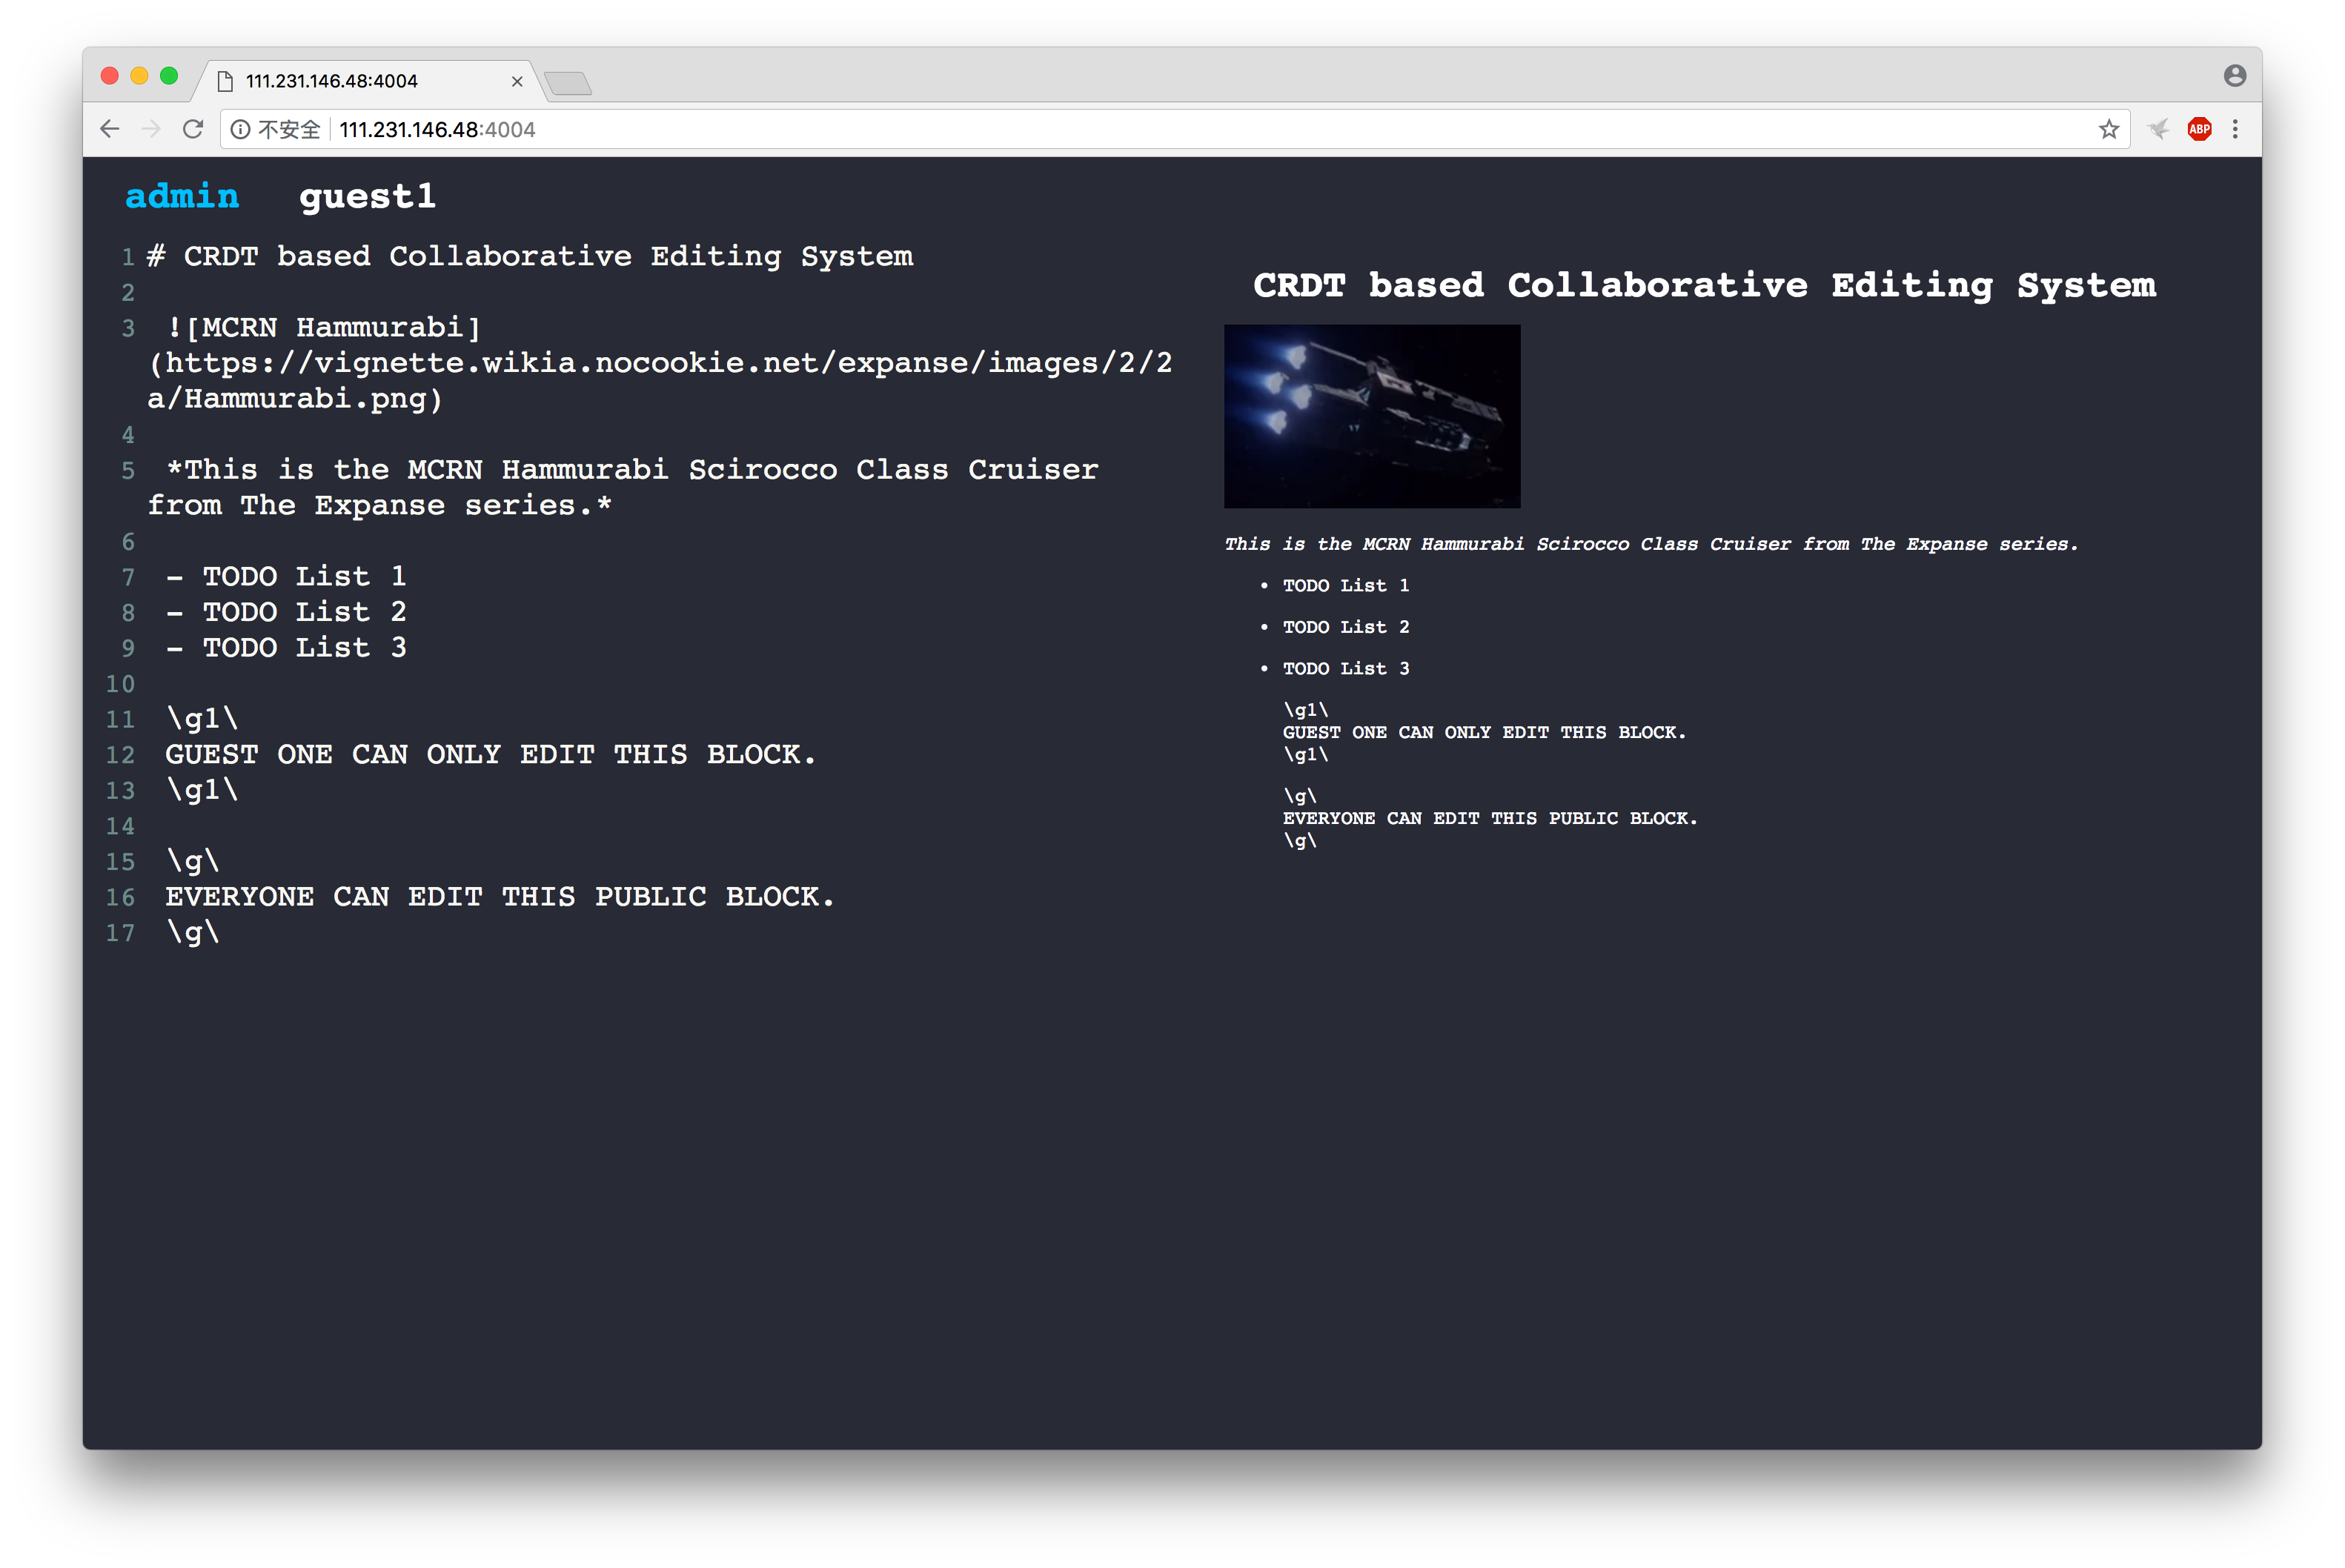
\includegraphics[width=\textwidth]{figures/demo.png}
    \caption{最终实现效果}
    \end{center}
\end{figure}
\section{背景知识}
本部分内容将介绍与此项目相关的背景知识,其部分内容在调研报告和可行性报告中也有所介绍,在此也对其中的关键内容进行一下回顾。
\subsection{实时文本协作的技术难点}
实时文本协作从用户层面来说看似十分简单,然而其面对的技术难题却是相当巨大的。业界在此问题上也进行了几十年的研究,最终也才在近些年来诞生了像Google Docs这样较为
完善的实时文本协作系统。其主要的难点在于解决不同用户的数据副本之间的同步问题。  

通常在这种高交互性的网络应用中,为了隐藏网络延时对用户体验带来的影响,我们要在每个客户端上
保存一个本地的用户副本。每个用户的操作都直接在本地数据副本上执行,这样本地的操作就不会受到网络延时的影响,用户能获得很好的本地响应性。
然而,这样的方式也会带来问题。需要设计一种机制维持各个用户的数据副本之间的一致性。如果用户的副本出现了不一致的情况,
那么显然会导致灾难性的后果。

我们用一个具体例子来说明其中的技术难题。假设现有Alice和Bob两人同时进行文档的编辑。
初始状态下Alice和Bob各自的副本都是相同的,内容如下:
\begin{center}
\textit{We wanted cars, instead we got characters.}
\end{center}

此时Alice想在 \textit{got} 后面插入 \textit{140} ,同时Bob又想在 \textit{wanted} 后面插入 \textit{flying}。
如果网络没有任何延时,所有的操作都能被瞬间应用,而Alice和Bob之间的操作在物理上也必然会有个先后关系,两者的操作会按照时间的先后关系而被执行,
这里我们就不会遇到任何问题了。
但是,由于网络有延时,那么问题就来了。Alice和Bob两个人各自都先执行自己的本地编辑操作,Alice先会进行一个 \textit{insert(140, col=30)} 的操作,在第30个位置插入
字符串 \textit{140} ,同样Bob先会执行的操作是 \textit{insert(flying, col=9)} 。此后,Alice和Bob分别将自己进行的操作广播给对方
Alice受到Bob的操作后然后执行 \textit{insert(flying, col=9)} ,Bob收到Alice的操作后执行 \textit{insert(140, col=30)} 。

此时,对Alice来说一切正常,她得到的状态是:
\begin{center}
    \textit{We wanted flying cars, instead we got 140 characters.}\footnote{Peter Thiel的名句,讽刺了人类似乎点错了科技树,近些年来除了互联网领域有飞跃性的进展,
    我们的科技缺少从0到1的突破。}
\end{center}

但Bob就糟糕了,此时Alice实际想要插入的位置就不是第30个位置了。Bob的状态变成了:
\begin{center}
    \textit{We wanted flying cars, instead 140 we got characters.}
\end{center}

显然,Alice和Bob得到了不一致的结果,这显然是文本协作中不能容忍的。为此,我们的核心问题就是通过一种什么样的机制来保证每个用户都能得到相同的数据副本?
\subsection{CRDT}
为了解决上述问题,业界也展开了数十年的研究,很多种方案例如AST(Address Space Transformation)、OT(Operational Transformation)、
WOOT(WithOut Operational Transformation)、CRDT(Conflict-free Replicated Data Type)被相继提出。
目前大多数主流文本协作应用例如Google Docs、石墨文档用的均是OT技术。OT的核心思想非常简单,当远程的操作到达本地站点后,其操作的上下文
可能和相应的客户端发出该操作时不同了,为了正确的执行该操作,我们要在执行远程操作之前对其转换,使得在当前的上下文下执行操作仍然不改变原始操作效果。
由于需要谨慎考虑所有可能出现的情况,OT不具备较好的可伸缩性,同时实现起来也非常复杂。CRDT则是近些年来新提出的一种技术,也正在逐渐被更加深入的研究
和在产品中应用。

CRDT有很多种不同的具体类型和实现,但大体上可以分为两类:基于状态的CRDT和基于操作的CRDT。基于状态的CRDT在更新时会将副本的
整个状态广播给其他副本。当一个副本收到了其他副本的状态时,会根据merge函数的机制和本地的状态进行merge。而基于操作的
CRDT则在每次更新时不广播整个副本的状态,而仅仅广播更新的操作,这样避免了整个状态过大不便于传输的问题。
\begin{figure}[ht]
    \begin{center}
    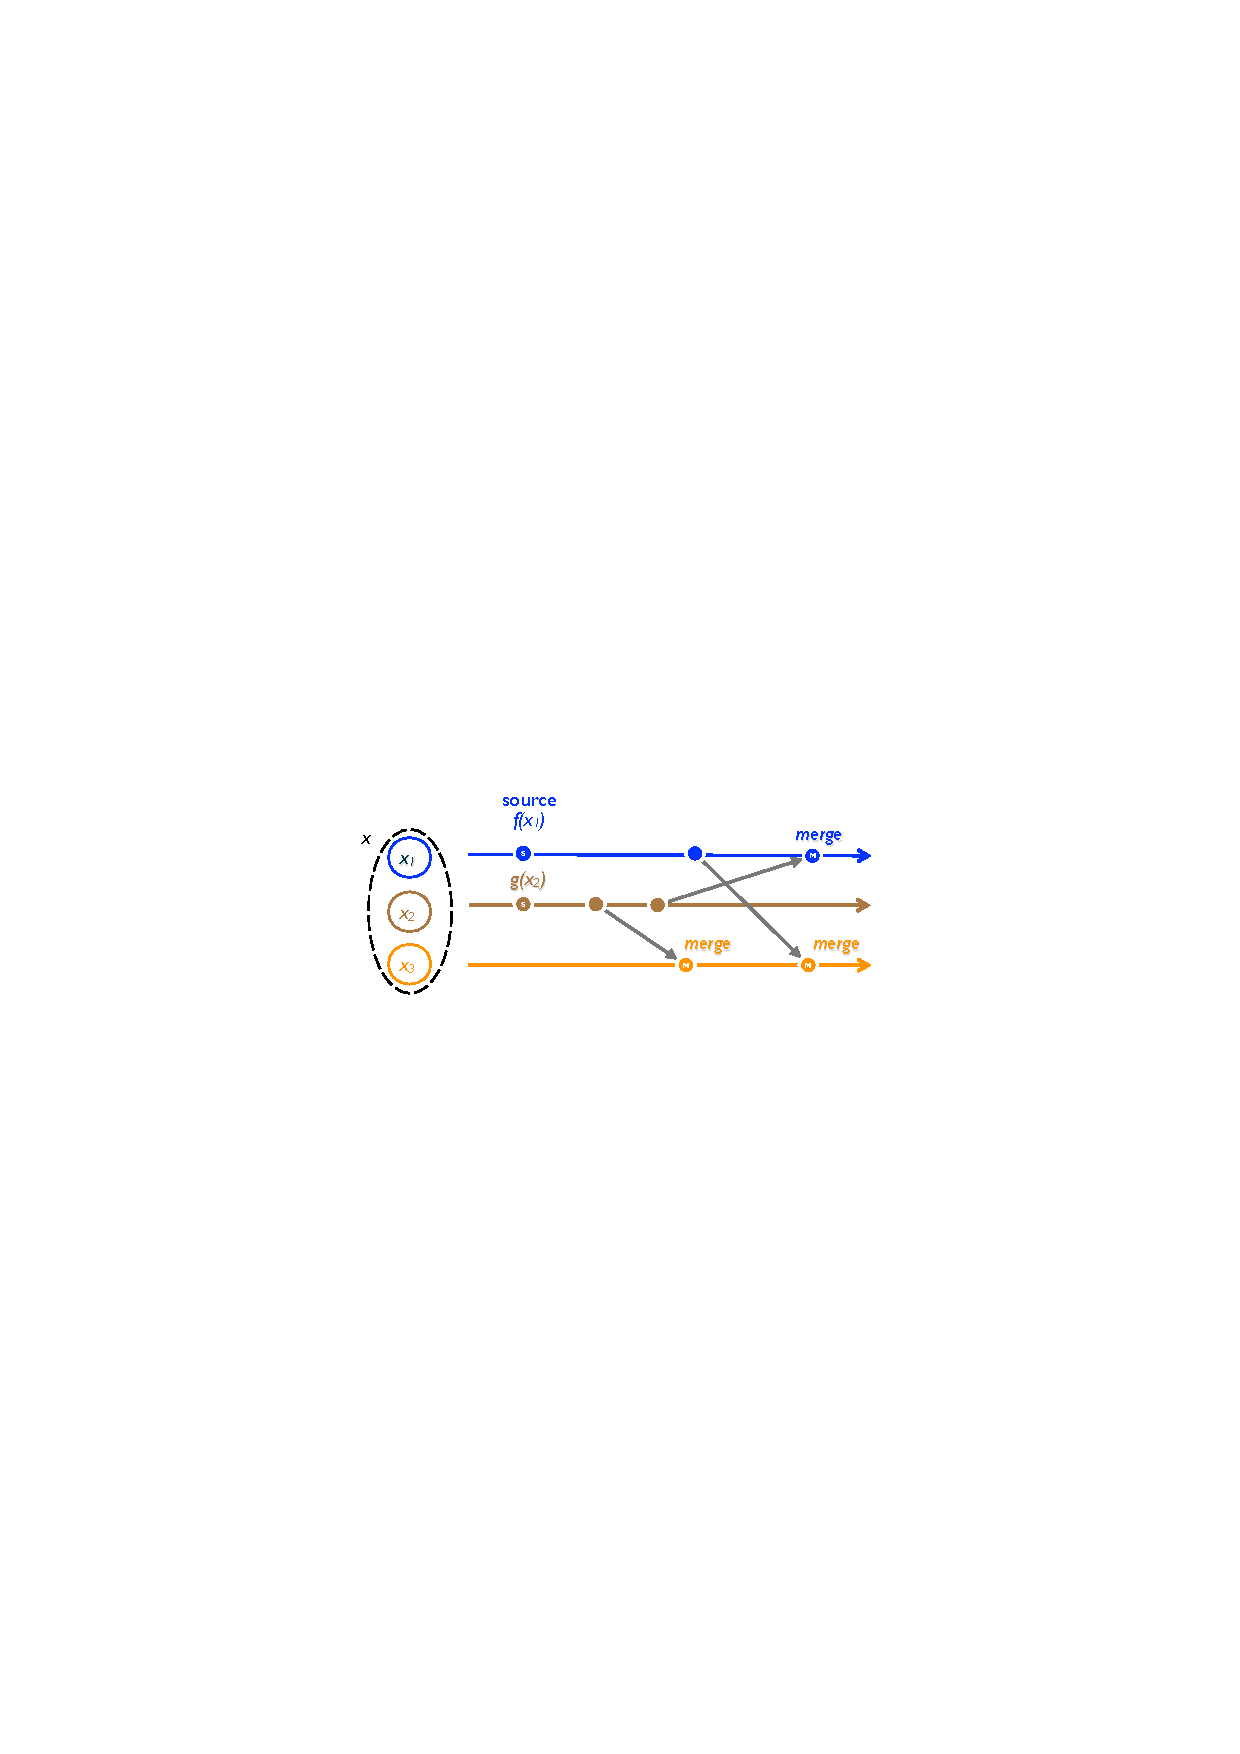
\includegraphics[width=\textwidth]{figures/state_crdt.pdf}
    \caption{基于状态的CRDT}
    \end{center}
\end{figure}

在该项目中我们采用了一种基于状态的CRDT实现文本协作,通过给文本中的每一个字符一个独一无二的标识符,我们将一个文本文档转换成了
一个有序的标识符序列。通过这个标识符序列,我们可以很轻松地维护各个副本之间一致性。CRDT这种数据类型能够使得并发操作之间相互commute。如果操作
是以先行发生(happen-before)的顺序产生,那么CRDT的副本之间不需要复杂的并发控制就能自动收敛达成一致。

在文本实时协作中,我们给每一个原子(也就是每一个字符)赋予一个独一无二的位置标识符(PosID),满足一下三条原则
\begin{enumerate}
	\item 每一个在缓冲区中的原子都有一个ID
	\item 任意两个不同的原子都有两个不同的ID
	\item 一个给定原子的ID在整个文档剩余的生命周期中保持不变
	\item ID之间有一个全序关系,和原子在缓冲区中的顺序一致
	\item ID取值空间是密集的,即:$\forall P, F : P < F \Rightarrow \exists N: P < N < F$
\end{enumerate}
我们定义一个抽象的原子数据缓冲区的状态T是一个由 (\textit{atom,PosID}) 二元组构成的集合,状态T的内容就是由T中所有原子按照\textit{PosID}排列构成的序列。 

每一个用户都会维持这个CRDT的一个副本,并且进行本地编辑
\begin{itemize}
	\item \textit{insert}($\mathit{PosID_{n}}$, newatom)
	\item \textit{delete}($\mathit{PosID_{n}}$)
\end{itemize}
这样,两个指向不同的PosID的操作是相互独立的。因为他们对于CRDT的作用效果是与他们的执行顺序无关的。那么现在只需要考虑并发的指向相同的PosID的两个操作。
一个插入操作必定发生在一个删除操作之前签,所以他们不可能是并发的。最后,删除操作是幂等的(idempotent),因为删除掉了一个给定PosID的字符再次删除这个PosID的字符是无效的。
因此,我们这样构建的一个缓冲区就构成了一个简单的CRDT,实现了文本实时协作功能。

但是,在这里还有两个问题需要考虑。
\begin{itemize}
	\item 两个客户端在同一时间生成了同样的PosID(当他们并行地在同一个位置插入字符)
	\item 一个客户端生成了一个已经被使用过的PosID(删除一个字符之后重新插入他们)
\end{itemize}

第二个问题很好解决,每个客户端自己只要维持一个记录,保证不会生成自己已经使用过的PosID即可。第一个问题同样可以用一个很简单的方法解决,我们只要将每一个PosID变成一个二元组即可,把PosID这个标识数字和产生该ID的客户端编号放在一起即可。这样就保证了两个客户端不会产生同样的PosID。
\subsection{Socket.IO}
Socket.IO是一个面向实时Web应用的JavaScript库,封装了WebSocket等协议实现了TCP客户端和服务器端全双工通信。
Socket.IO提供了一个相当高级的接口,其使用起来也极为简单。
在客户端,只需要在HTML文件中引入Socket.IO脚本即可,只需要一行代码
\begin{minted}{html}
    <script src="/socket.io/socket.io.js"></script>
\end{minted}

服务器端所需要的操作也很简单
\begin{minted}{javascript}
    var io = require("socket.io").listen(server);
\end{minted}
就可以将socket.io绑定到服务器上,任何连接到该服务器上的客户端都具备了实时通信功能。

然后使用
\begin{minted}{javascript}
    io.on("connection", function (socket) {...}
\end{minted}
就可以监听所有客户端,返回新的连接对象(socket即为连接对象)。

Socket.IO是事件驱动的,其核心操作也就是广播一个事件和监听事件并相应,
主要通过\textsf{socket.emit(eventName[, ...args][, ack])}和\textsf{socket.on(eventName, callback)}
两个函数来实现
\textsf{emit}函数广播一个事件,第一个参数为事件的名字,之后可选为传递的参数,\textsf{ack}为可选参数,服务器应答时会调用该函数。
\textsf{on}函数用来监听一个事件,相当于系统中的一个signal handler,这个函数为指定的事件绑定一个handler,第一个参数为事件的名字,
第二个参数为handler。

\section{详细设计}
\subsection{主体架构}
\begin{figure}[ht]
    \begin{center}
    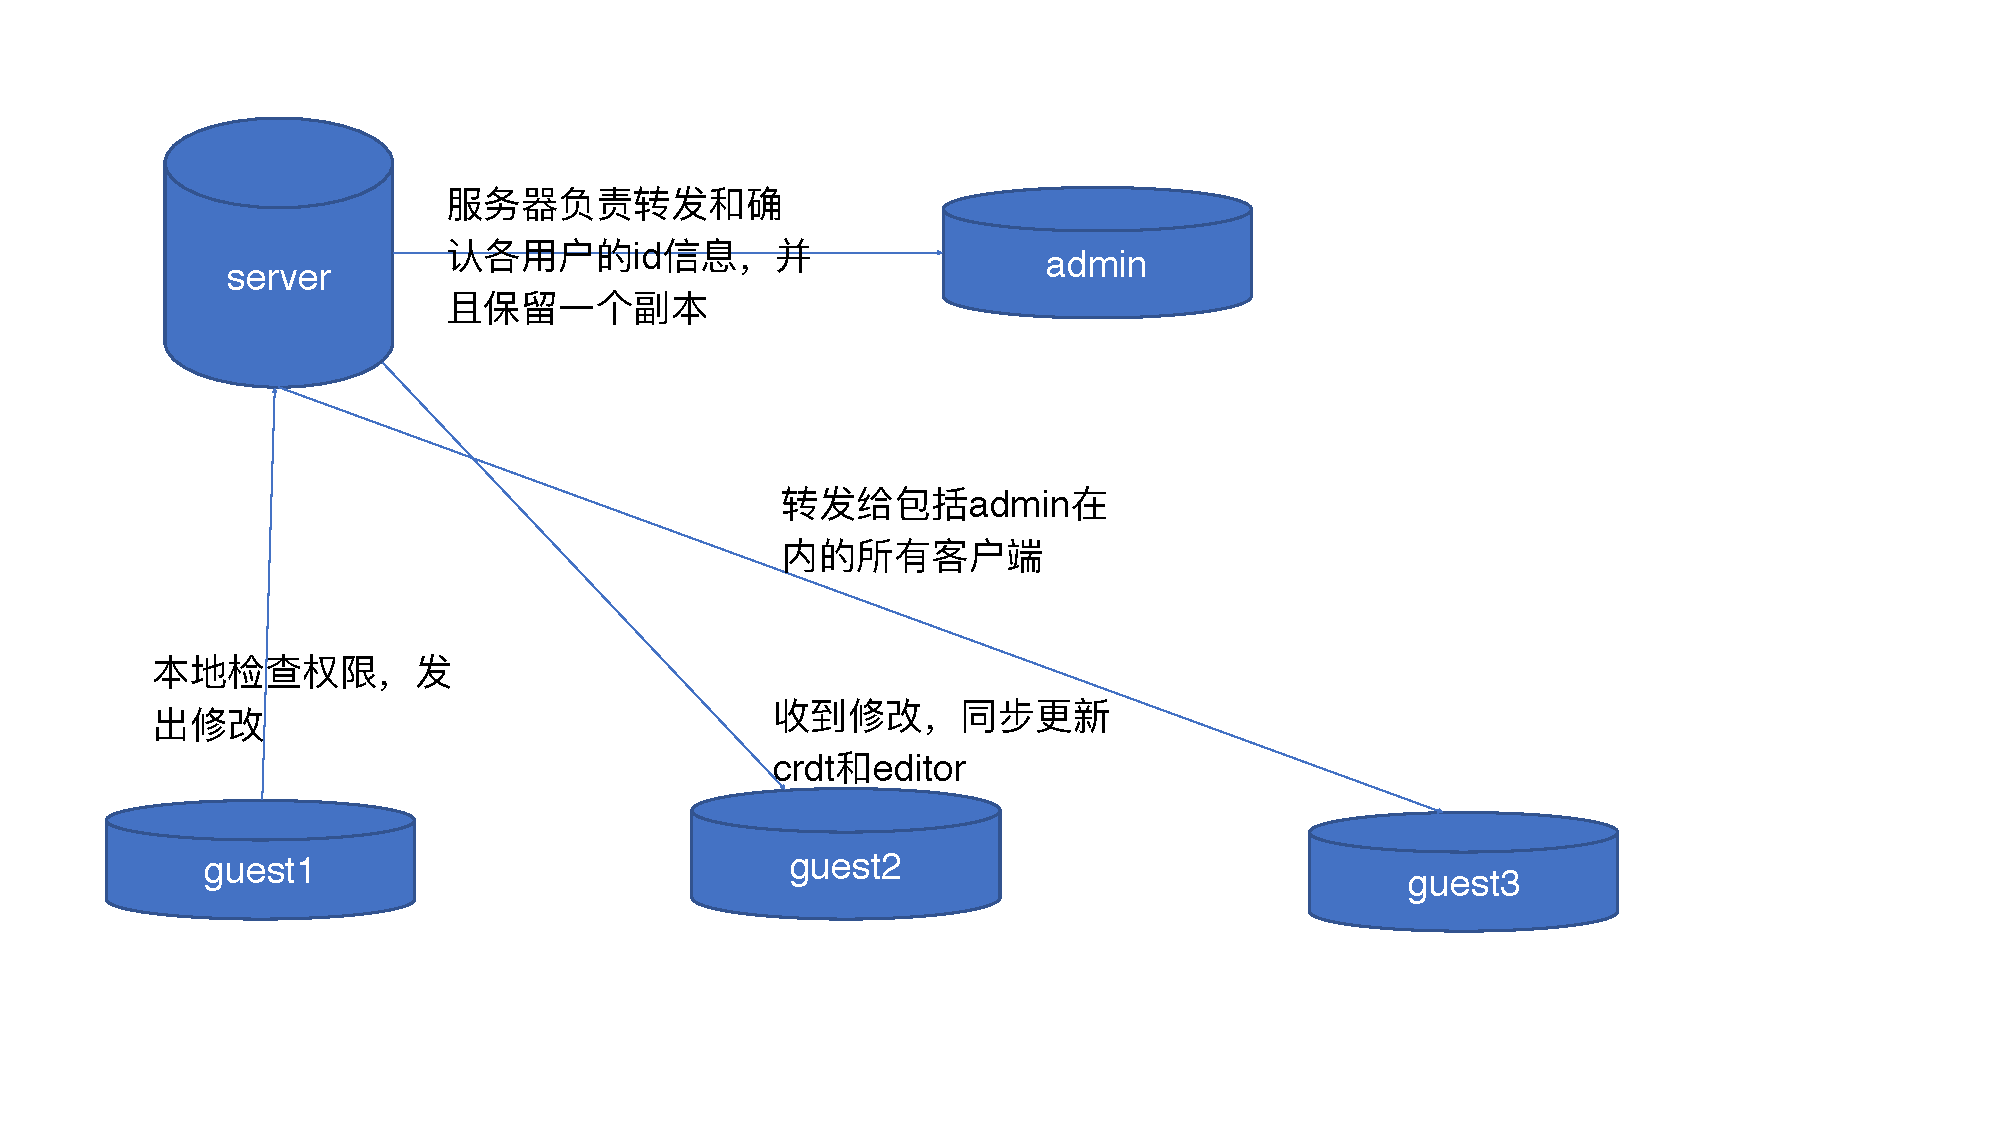
\includegraphics[width=\textwidth]{figures/arch_1.pdf}
    \caption{Client-server model}
    \end{center}
\end{figure}
\begin{figure}[ht]
    \begin{center}
    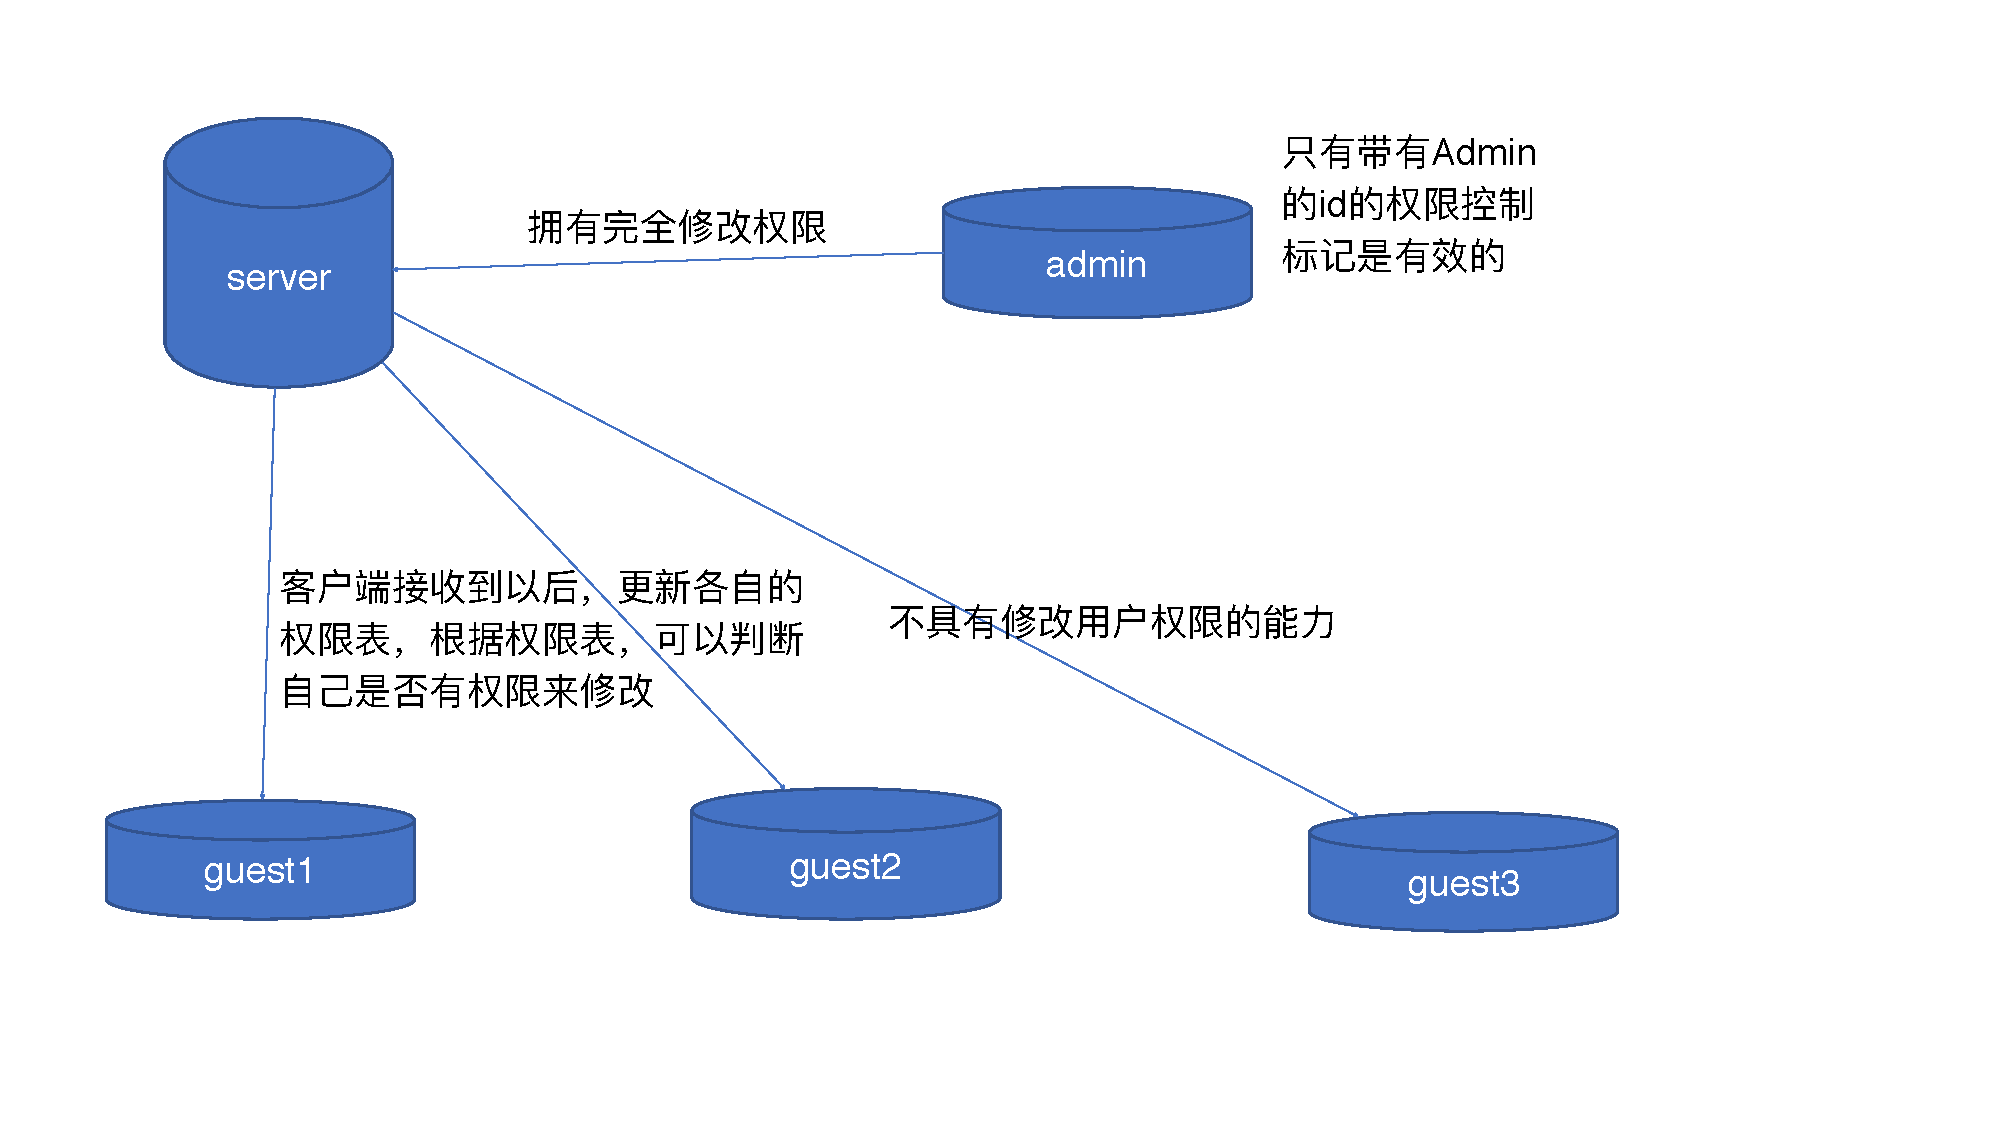
\includegraphics[width=\textwidth]{figures/arch_2.pdf}
    \caption{权限控制设计}
    \end{center}
\end{figure}
图3和图4分别说明了本项目的客户端-服务器模型的基本架构以及权限控制的具体机制。

我们采用了Node.js作为后端部署在服务器上运行,借助npm包管理器,服务器程序可以轻松部署在任何一台服务器上。\textsf{package.json}中给出了
相应的包依赖关系,使用如下两条命令即可完成服务器端的部署:
\begin{minted}{shell}
npm install
node app.js
\end{minted}

默认监听4004端口,可以在\textsf{app.js}中更改。

服务器在我们的设计中仅负责转发和确认用户的ID信息,并且保留一个副本给新加入的编辑者提供初始状态。本身基于CRDT的实时协作架构是可以用完全去中心化的点对点网络实现,
但使用客户端-服务器的模型可以简化我们的工作,同时也便于实施权限控制。权限的检查我们采用在客户端本地进行。当客户端检查确认自己有权限编辑某一段时,才会发出修改请求。
由于本项目的定位为提供一个用于技术团队在同一局域网下的文本实时协作,我们不考虑恶意攻击者的情况。恶意攻击者可以通过修改客户端跳过权限检查来实现作弊。但将权限的判断移植到
服务器端也是可行的,而且也并不困难。

\subsubsection{权限管理的具体机制}
\begin{itemize}
    \item 用户分为admin与guest,admin是唯一的,其余为guest;
    \item 第一个登陆的人自动设为admin,一旦admin退出(离线),admin按顺序继承给下一个guest
    \item admin拥有完全编辑权限,并可划分区域,区域格式为\textsf{\textbackslash g\{i\}\textbackslash \ \textbackslash g\{i\}\textbackslash},i代表guest\{i\},即guest\{i\}只能在该区域中间(不包括区域标识符)编辑
    \item 每个guest在自己的编辑区域中再插入\textsf{\textbackslash g\{i\}\textbackslash \ \textbackslash g\{i\}\textbackslash}企图划分出一个层次性的编辑区域是无效的,也无法在命令区域中插入一个\textsf{\textbackslash g\{i\}\textbackslash}表示编辑区域的开始,而admin或其他人
    s在该guest的编辑区之外插入另一个\textsf{\textbackslash g\{i\}\textbackslash}表示编辑区域的结尾而划分编辑区域。只有admin能设置权限;
    \item \textsf{\textbackslash g\textbackslash \  \textbackslash g\textbackslash}表示公共编辑区域,任何人都可以在这一个区域中进行编辑。
\end{itemize}

\subsection{基于状态的CRDT的设计}
在本项目中,正如背景知识一节所介绍的一样,我们编写了一个基于状态的CRDT以实现各客户端副本之间的同步。在这一节里我们将介绍所使用的CRDT的具体设计。
\subsubsection{数据结构}
\paragraph{\textsf{identifier}}
文档中每一个字符所对应的位置标识符(position identifier)就是由一系列identifier类型构成的,每一个identifier是由一个数字标识digit(我们取256进制)和一个客户端ID的标识符site构成的二元组
\begin{minted}{javascript}
    C.identifier = (digit, site) => {
        return {
            digit : digit || 0,
            site : site || 0
        };
    };
\end{minted}

由这样一些列二元组组成的有序多元组就是一个字符的position identifier。对于不同的position identifier我们可以定义一个大小关系

对于每个identifier的比较,先看第一个元素,也就是digit,如果相等再比较第二个元素(客户端标识符)
\begin{minted}{javascript}
    C.compareIdentifier = (i1, i2) => {
        if (i1.digit < i2.digit) {
            return -1;
        } else if (i1.digit > i2.digit) {
            return 1;
        } else {
            if (i1.site < i2.site) {
                return -1;
            } else if (i1.site > i2.site) {
                return 1;
            } else {
                return 0;
            }
        }
    };
\end{minted}

对于整个position identifier的比较,采用类似字符串比较的方式,逐个identifier比较直到第一个不同的位置。如果公共部分相同,那么就看两个position identifier长度的不同。
\begin{minted}{javascript}
    C.comparePosition = (p1, p2) => {
        for (let i = 0; i < Math.min(p1.length, p2.length); i++)
        {
            let comp = C.compareIdentifier(p1[i], p2[i]);
            if (comp !== 0)
                return comp;
        }
        if (p1.length < p2.length) {
            return -1;
        } else if (p1.length > p2.length) {
            return 1;
        } else {
            return 0;
        }
    };
\end{minted}

\paragraph{\textsf{char}} 在CRDT中,我们的字符类型就是对文档中的普通字符和position identifier放在一起做了个封装,每个char由三个元素组成,一个position identifier(也就是identifier构成的数组),一个Lamport时钟(Lamport
时钟是一种逻辑时钟而非物理时钟,其主要用于在分布式系统中确定事件发生的顺序,其并不用于CRDT中的比较),以及字符的值。
\begin{minted}{javascript}
    C.char = (identifiers, lamport, value) => {
        return {
            position : identifiers || [],
            lamport : lamport || 0,
            value : value || ''
        };
    };
\end{minted}

\subsubsection{API}
我们设计的CRDT提供了以下API函数
\begin{minted}{javascript}
    C.add = (n1, n2)
    C.subtract = (n1,n2)
    C.fromIdentifiers = (identifiers)
    C.toIdentifiers = (num, before, after, site)
    C.increment = (num, delta)
    C.compareIdentifier = (i1, i2)
    C.equalChar = (c1, c2)
    C.comparePosition = (p1, p2)
    C.compareChar = (c1, c2)
    C.generatePositionBetween = (p1, p2, site)
    C.binarySearch = (U, V, comparator, notFoundBehavior)
    C.getChar = (lineIndex, charIndex)
    C.getCharValue = (lineIndex, charIndex)
    C.getLine = (lineIndex)
    C.compareCharWithLine = (char, line)
    C.findPosition = (char)
    C.getPreChar = (lineIndex, charIndex)
    C.updateCrdtRemove = (change)
    C.updateCrdtInsert = (lamport, site, change)
    C.remoteInsert = (char)
    C.remoteDelete = (char)
    C.convertLocalToRemote = (lamport, site, change)
    C.updateAndConvertRemoteToLocal = (change)
    C.isNumber = (ch)
    C.findAllAvailSpace = (site)
    C.isAvail = (availSpaces, char)
\end{minted}

接下来将重点介绍比较重要的几个函数
 
\subsubsection{\textsf{generatePositionBetween}}
\begin{minted}{javascript}
    C.generatePositionBetween = (p1, p2, site)
\end{minted}

这一函数可以算是CRDT中最关键的一个函数,它用递归算法来给给定客户端\textsf{site}生成一个介于\textsf{p1}和
\textsf{p2}之间的position identifier。其主要过程可以分为三种情况
\paragraph{情形一 —— p1和p2中第一个identifier的digit相同}
此时可以做到生成一个新的position identifier,position identifier的大小介于p1和p2之间,
而与p1和p2第一个identifier对应的site无关。只需要将p1的第一个identifier的digit增加一个
微小的量即可。为此,我们先扔掉p1和p2的每个identifier中的site,然后将其转换成十进制数字表示
\begin{minted}{javascript}
    let n1 = C.fromIdentifiers(p1);
    let n2 = C.fromIdentifiers(p2);
\end{minted}
然后进行加减法,最后转换回数组形式的position identifier
\begin{minted}{javascript}
    let delta = C.subtract(n2, n1);
    let next = C.increment(n1, delta);
    return C.toIdentifiers(next, p1, p2, site);
\end{minted}

\paragraph{情形二 —— p1和p2第一个identifier的digit相同,但site不相同}
假设p1第一个identifier的site是x,p2是y。并且假设x小于y。那么我们只要让新生成的position identifier的
第一个identifier的digit和p1以及p2第一个identifier相同,而site=x,那么新生成的position identifier就一定小于p2。递归调用
\begin{minted}{javascript}
    return 
    [head1].concat(
    C.generatePositionBetween(rest(p1), [], site)
    );
\end{minted}

注意我们将p2替换成了[],因为新的position identifier的后半截只要比p1的后半截大即可,而没有小于的要求。
\paragraph{情形三 —— p1和p2第一个identifier的digit和site都相同}
递归调用
\begin{minted}{javascript}
    return 
    [head1].concat(
    C.generatePositionBetween(rest(p1), rest(p2), site)
    );
\end{minted}

\subsubsection{\textsf{updateCrdtRemove}}
\begin{minted}{javascript}
    C.updateCrdtRemove = (change)
\end{minted}

在看本函数之前,先介绍一下\textsf{change}这个对象是什么。我们前端的实现采用了CodeMirror这一网页文本编辑器。
CodeMirror也是采用事件响应的。当编辑器的内容被修改时,编辑器就会立刻发出一个\textsf{"change" (instance: CodeMirror, changeObj: object)}的事件,\textsf{changeObj}
描述了文本的变化,其是一个\textsf{\{from, to, text, removed, origin\}}这样的对象,from和to是一个二元组对象,包含了\textsf{\{ch, line\}},是一个二维坐标,
通过一个字符所在的行和相对于这行的位置指明了一个字符。from和to分别代表修改的起始位置和截止位置。text为修改后的文本,removed为修改前的文本,这个文本已经被text给替换掉了
origin参数决定了选择历史事件可不可以被合并到之前的操作。

本函数(\textsf{updateCrdtRemove})函数实现的是对\textbf{本地}CRDT副本实现删除操作,函数仅需要一个参数change。
首先函数会根据传递进来的change参数来确定需要删除的行有哪些。
然后针对每行确定删除的起始位置和截止位置。对于第一行来说,删除的开始位置在change中指定,然后一直删除到该行末尾。
中间的所有行都是从头删到尾,然后最后一行从头删除到change中给定的位置。
函数执行实际的删除操作,同时将删除了的内容返回。
\subsubsection{\textsf{updateCrdtInsert}}
\begin{minted}{javascript}
    C.updateCrdtInsert = (lamport, site, change)
\end{minted}

这个函数用于执行\textbf{本地}CRDT副本的字符插入。每次插入操作会在两个相邻的字符中间插入一串字符。
首先先获得需要插入的行,获取插入位置前的字符,插入位置之后的字符。针对每一个要插入的字符生成一个新的position identifier(调用
\textsf{generatePositionBetween}函数),然后用这个position identifier生成一个新的我们定义的char类型的对象,将这个char加入到
在插入位置之前的字符数组before。如果遇到了换行符,那么就用before中的字符生成一个新的行,将新行加入到行数组lines中,同时清空before中的内容。
最后再将before和插入位置之后的字符构成的数组after相连接,形成最后的一行。函数返回插入的字符。

\subsubsection{\textsf{remoteInsert}}
\begin{minted}{javascript}
    C.remoteInsert = (char)
\end{minted}

该函数是用来合并远程的插入操作,这个函数的参数是一个我们封装的char类型,我们只需要查找到对应的位置,然后发出一个相应的change对象给
CodeMirror文本编辑器。如果插入的这个字符是换行符,那么需要做一个特别的处理,拆分出换行符之前和之后的字符,形成两个新的行。
\subsubsection{\textsf{remoteDelete}}
\begin{minted}{javascript}
    C.remoteDelete = (char)
\end{minted}

该函数用来合并远程删除,其和处理远程插入一样,只要一个char类型作为参数。找到对应的位置并且发出合适的change对象。
如果遇到了换行符,那么需要把当前行和下一行合并。这个操作也并不困难,只要构造一个这样的change对象即可
\begin{minted}{javascript}
    from : {line: lineIndex, ch}, 
    to : {line: lineIndex + 1, ch: 0}, 
    text : ""
\end{minted}

\subsubsection{\textsf{findAllAvailSpace}}
\begin{minted}{javascript}
    C.findAllAvailSpace = (site)
\end{minted}

这个函数是权限控制功能的主要构成部分。我们CRDT的整个文档信息以char数组的形式保存在\textsf{C.crdt}中,我们可以以二维数组
按行和对应行的位置来索引字符。该函数用来寻找给定客户端(通过客户端标识符参数\textsf{site}传递)能编辑的文档范围。首先,
逐行逐字符搜寻,直到找到匹配的权限控制标识符\textsf{\textbackslash g\{i\}\textbackslash}或\textsf{\textbackslash g\textbackslash}
(公共编辑区域)。针对第一种情况,提取guest的编号保存在\textsf{num\_site}变量中。此后通过相应的标识符来判断当前的权限控制符是
标志区域的开始还是结尾。如果遇到了结尾标识符,那我们就确定了一个对应用户的可以编辑区域。如果这个用户和通过参数传递过来的想要查询可行域的
用户相同,那么就把这个区域加入到可行域的集合中去,否则不理会。我们的算法设计也使得遇到了第一个区域开始标识符后,会找到与之
相匹配的第一个区域结尾标识符,而不理会这个区域中间的其他任何标识符,也因此保证了只有admin能够实现权限的控制。

\subsection{服务器设计}

\clearpage

\nocite{*}
\bibliographystyle{plain}
\bibliography{ref}
\end{document}